\relatorio
{O mercado brasileiro de corridas de montanha}
{
    \noindent Pesquisadores: Iara Vivian e Henrique Puppi
    
    \noindent Orientador: Neto Concon
}
{
   O projeto tem como objetivo realizar um estudo sobre o mercado de *trail running* brasileiro, através da construção de um banco de dados com informações relevantes para o mercado de corrida de montanha no Brasil. Dessa forma, será possível entender as proporções desse mercado atualmente e traçar o perfil do corredor de montanha no Brasil.
}
{
    Construção de base, corrida de montanha
}

\section{Introdução}

A corrida de montanha (ou trail running) é uma vertente da corrida tradicional praticada fora dos ambientes urbanos, como: serras, montanhas e trilhas. Essa modalidade tem crescido no mundo, conforme mostrado na Figura \ref{fig:logo}.

\begin{figure} [H]
    \centering
    \caption{Número de corridas ao longo dos anos no mundo.}
    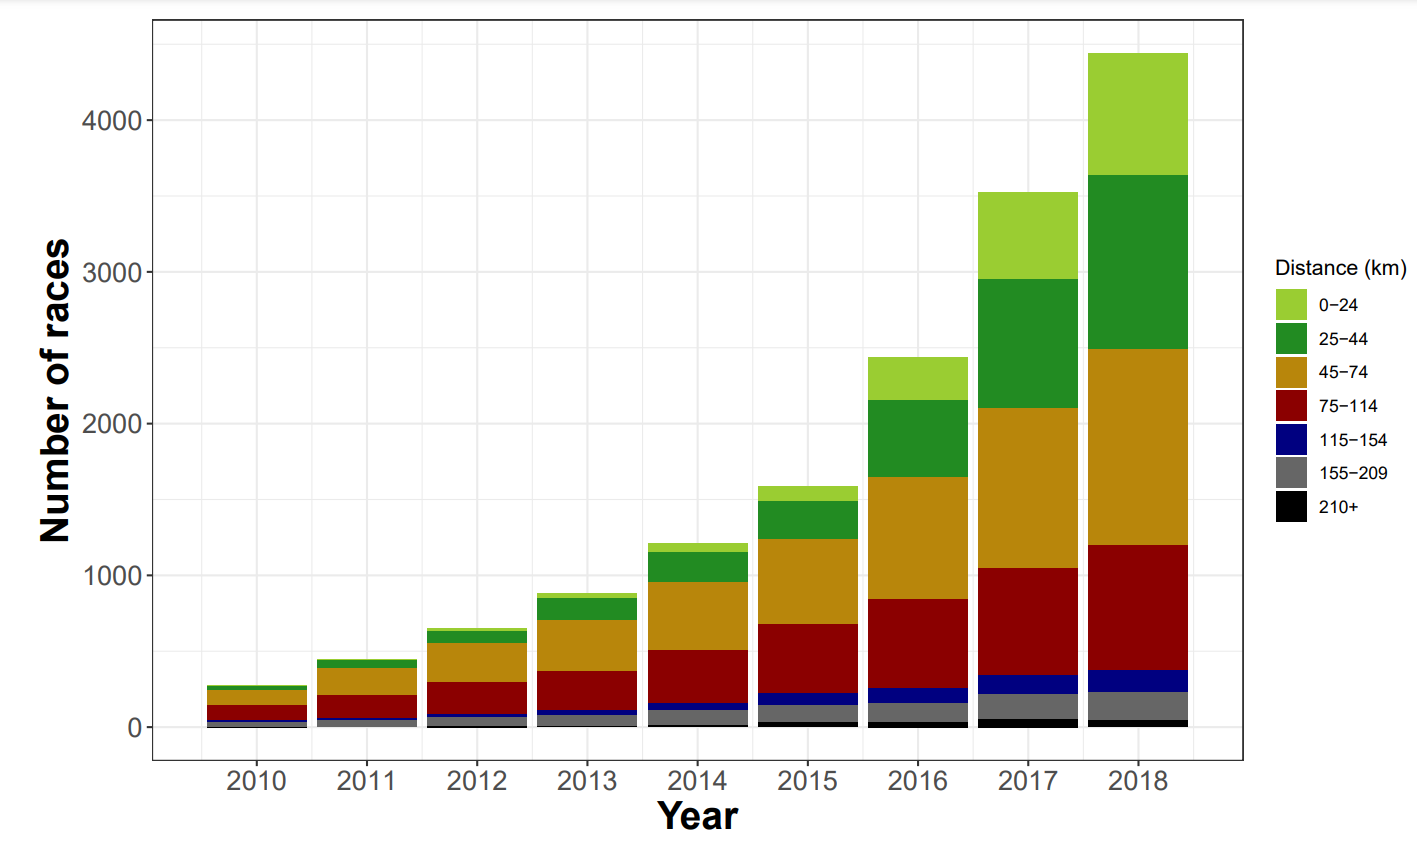
\includegraphics[width = 0.9\linewidth]{relatorios/paraty/figuras/image1.png}
    \label{fig:logo}
\end{figure}

Já no Brasil, a corrida de montanha ainda é pouco difundida se comparada a outros países que já tradicionalmente a praticam, como evidenciado pela Figura \ref{fig:imagem1}.


\begin{figure}
    \centering
    \caption{Distribuição geográfica das corridas pelo mundo.}
    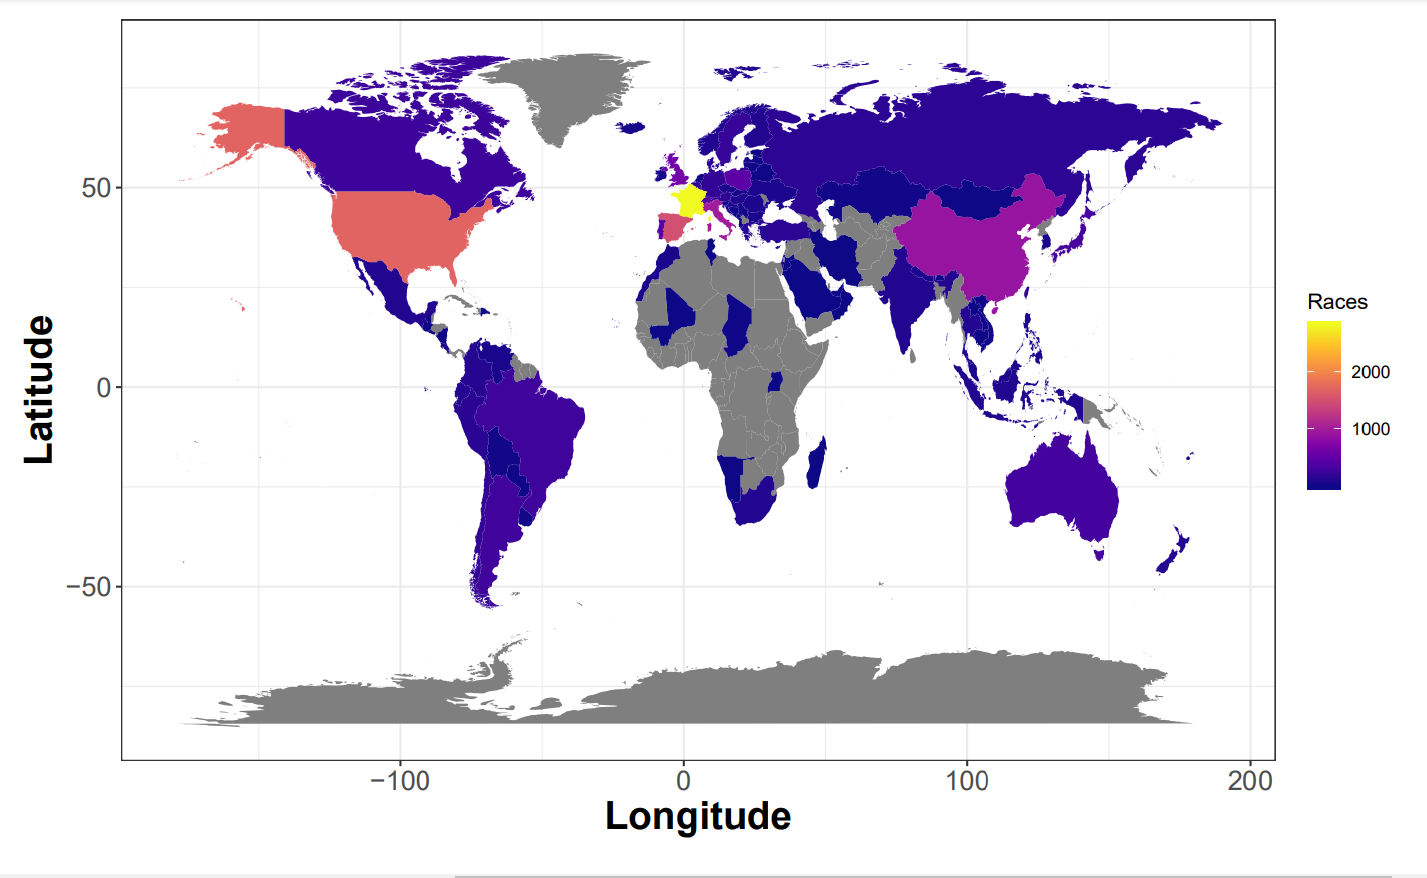
\includegraphics[width = 0.9\linewidth]{relatorios/paraty/figuras/image3.png}
    \label{fig:imagem1}
\end{figure}

 Em outubro de 2016, o Brasil participou pela primeira vez do Campeonato Mundial de Trail Running (Trail World Championship – TWC) que foi realizado em Portugal, a delegação brasileira contou com 6 atletas que competiram contra as outras 39 delegações presentes, somando um total de 302 corredores na competição (ULTRA TRAIL DU MONT BLANC, 2016). Ademais, também em 2016, 90 atletas brasileiros participaram do maior evento de trail running do mundo, o Ultra Trail du Mont Blanc (UTMB), que ocorre anualmente na França, Itália e Suíça, que contava na época com mais de 8000 corredores por ano \cite{oliveira2017}.

Apesar do crescimento da modalidade no Brasil, ainda são escassas as pesquisas realizadas sobre o assunto, dificultando, assim, a exploração desse mercado novo que se expande pelo país. Segundo Daniel Ramos, o seu artigo foi o primeiro relacionado à trail running escrito em língua portuguesa e, essa carência de materiais a respeito do mercado, acarreta uma dificuldade para criar competições e circuitos ao redor do país pois organizadores de corridas brasileiros precisam de uma estimativa de participantes para ter rentabilidade econômica, uma vez que é necessário alugar local, comprar garrafas de água, equipamentos, faixas etc. Além disso, a falta de informação prejudica os próprios atletas a encontrarem provas futuras para participarem (Daniel JUNIOR, 2017).

O UTMB apresentou em seu portfólio a Paraty Brazil, primeiro circuito oficial do esporte no Brasil, que ocorreu entre os dias 22-24 de Setembro de 2023 (ULTRA TRAIL DU MONT BLANC, 2023). Hoje a UTMB conta com 4 corridas no Brasil, todas promovidas pela Paraty, porém com diferentes quilometragens (duas de 20 km, uma de 50 km e uma de 100 km), e com aproximadamente 36,6 mil corredores brasileiros registrados no site. 

De acordo com Neto Concon, CSO e corredor da Paraty Brazil, uma das maiores dificuldades de organizar um circuito de trail running no Brasil é a expectativa numérica de participantes. O CSO também mencionou situações em que as vagas disponibilizadas e esperadas para uma corrida foram preenchidas em menos de 1 semana, mostrando um exemplo da falta de pesquisa de mercado.

\begin{figure}
    \centering
    \caption{Corrida Paraty Brazil 2023}
    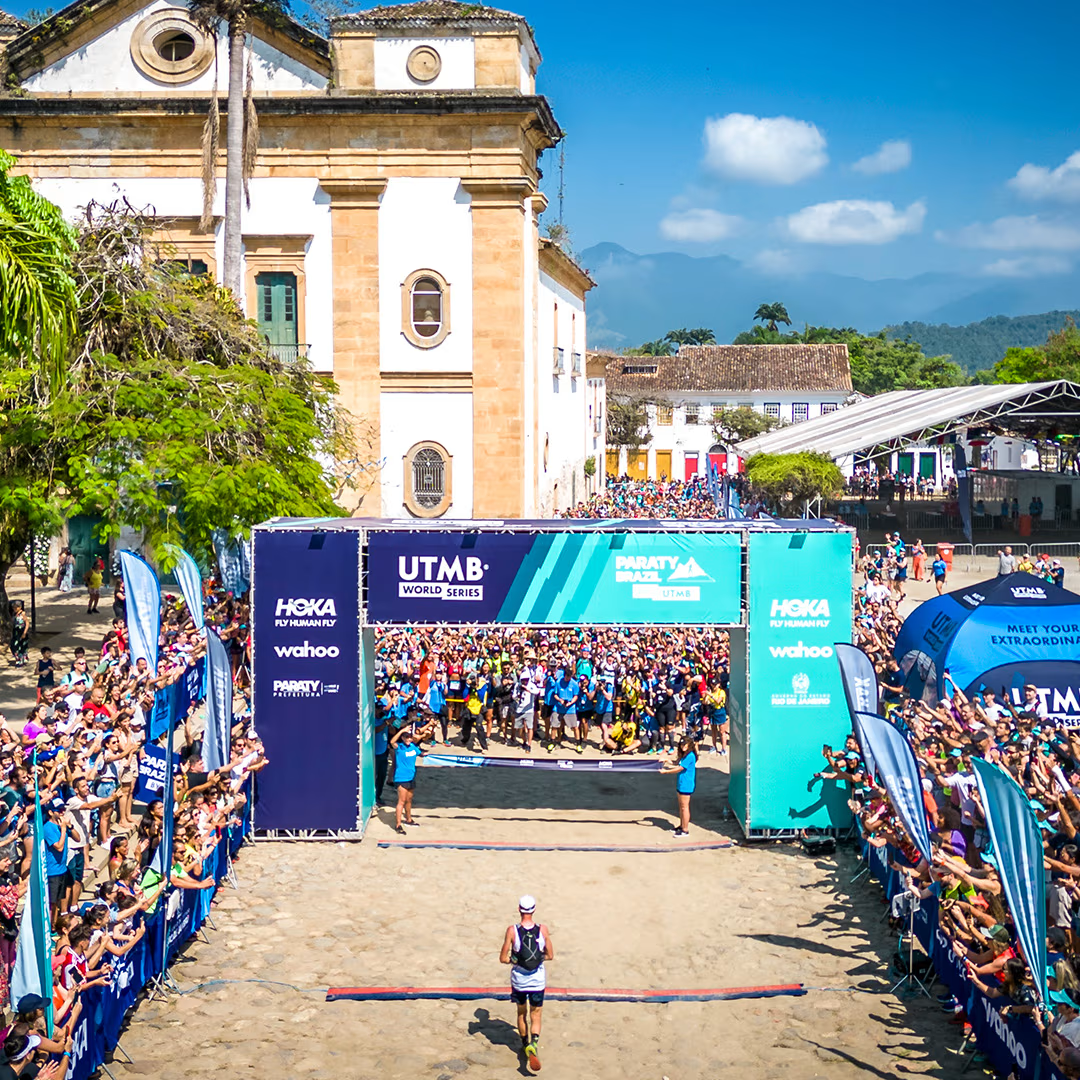
\includegraphics[width = 0.5\linewidth]{relatorios/paraty/figuras/image4.png}
    \label{fig:paraty}
\end{figure}

Assim, o presente artigo tem como objetivo realizar um estudo sobre o mercado de trail running brasileiro, através da construção de um banco de dados com informações relevantes para o mercado de corrida de montanha no Brasil. Dessa forma, será possível entender as proporções desse mercado atualmente e traçar o perfil do corredor de montanha no Brasil.

\section{Desenvolvimento}

\subsection{Revisão Literária}

A construção de uma base de dados para auxiliar a análise do mercado de corridas de montanha no Brasil é um empreendimento novo, e que exige um entendimento das práticas de pesquisa de mercado. Por ser um mercado novo e crescente na cultura brasileira, não há indícios de uma central de informações estruturada, e essa é a lacuna a ser preenchida.

Segundo o livro "Market Research in Practice" de Paul Hague, Matthew Harrison, Julia Cupman e Oliver Truman, a pesquisa de mercado é fundamental para coletar dados relevantes que ajudam a entender melhor o comportamento dos consumidores, identificar tendências e oportunidades, e tomar decisões estratégicas informadas. Este livro destaca a importância de uma abordagem metódica e sistemática na coleta e análise de dados, enfatizando que a precisão e a relevância das informações coletadas são cruciais para o sucesso de qualquer análise de mercado \cite{hague2021}.

O trabalho de Hague et al. \cite{hague2021} ressalta que uma pesquisa de mercado eficaz deve começar com uma definição clara dos objetivos de pesquisa e uma compreensão detalhada do mercado-alvo. A coleta de dados pode envolver uma combinação de métodos quantitativos e qualitativos, como pesquisas, entrevistas, e análise de dados secundários disponíveis. A metodologia recomendada no livro, pode ser aplicada diretamente à iniciativa de construção de uma base de dados, garantindo que a coleta de informações seja abrangente e precisa.

Complementando essa perspectiva, o artigo "Pesquisa de Mercado" de Hélvio de Avellar Teixeira (UFMG) enfatiza a importância da pesquisa de mercado na identificação de oportunidades e ameaças no ambiente competitivo. Teixeira \cite{teixeira2012} argumenta que a pesquisa de mercado é uma ferramenta estratégica essencial, auxiliar à qualquer organização que deseja se posicionar de forma eficaz no mercado. No caso do mercado de corridas de montanha, a pesquisa pode revelar insights valiosos sobre as preferências dos corredores, os fatores que influenciam suas escolhas de eventos, e as lacunas no mercado que podem ser exploradas para desenvolver novos serviços ou melhorar os existentes.

Teixeira \cite{teixeira2012} também destaca a necessidade de uma análise cuidadosa dos dados coletados, para garantir que as conclusões tiradas sejam válidas e aplicáveis. Ele sugere que, o uso de técnicas estatísticas e ferramentas de análise de dados, pode melhorar significativamente a qualidade das inferências feitas. Este ponto é particularmente relevante para o projeto, pois a construção de uma base de dados completa, e a aplicação de análises, permitirão a identificação de padrões e tendências que podem não ser imediatamente evidentes.

Para a construção de uma base de dados para análise do mercado de corridas de montanha no Brasil, deve-se seguir uma rota metodológica detalhada, conforme recomendado pela literatura especializada em pesquisa de mercado. Segundo o livro de Hague et al. \cite{hague2021}, a estruturação deve começar com o dimensionamento do mercado, coletando dados imprescindíveis para a exploração. Hélvio de Avellar Teixeira, no artigo "Pesquisa de Mercado", enfatiza a importância de identificar as necessidades dos enolvidos, para aumentar a eficiência do processo \cite{teixeira2012}. Questões de pesquisa específicas para a coleta de dados também são essenciais, uma coleta sem alvo não fornece ajuda. Após a coleta, utilizam-se técnicas estatísticas para análise, garantindo que as conclusões sejam válidas e aplicáveis. A etapa final envolve a integração dos dados coletados na construção de uma base de dados completa e acessível, que será mantida e atualizada regularmente, conforme recomendado por Hague et al. \cite{hague2021}.

\subsection{Análise teórica}

A organização de um evento de corrida de
montanha envolve uma série de fatores econômicos
que são essenciais para o sucesso do evento.
Entre esses fatores, destaca-se a necessidade de
uma infraestrutura adequada, que inclui inclui a
instalação de aid stations, que são pontos de
apoio ao longo do percurso onde os corredores
podem reabastecer-se com água, alimentos e
receber assistência médica, caso necessário.

Além das aid stations, a organização de uma
corrida de montanha exige a aquisição de
equipamentos diversos e a implementação de uma
infraestrutura que garanta a segurança e a
experiência dos participantes. Devido à natureza
desses eventos, realizados em trilhas e
ambientes montanhosos, é imprescindível uma
sinalização clara e adequada, além de medidas de
segurança adicionais para mitigar os riscos
associados ao terreno.

Para garantir a viabilidade econômica do evento,
é fundamental um planejamento detalhado,
incluindo a estimativa do consumo de água por
participante, por exemplo. Com base no número
esperado de competidores, a organização pode
calcular a quantidade necessária de garrafas de
água a serem adquiridas, evitando assim
desperdícios e prejuízos financeiros.

Nesse contexto, a análise das variáveis
envolvidas torna-se crucial para a compreensão
do mercado de corridas de montanha. As variáveis
estudadas neste trabalho serão utilizadas em
análises posteriores e podem ser divididas em
duas categorias principais: as relacionadas aos
corredores e as relacionadas às corridas. As
variáveis relacionadas aos corredores incluem
faixa etária, nome completo, URI (Identificador
Uniforme de Recurso), nacionalidade, sexo, time,
patrocinador, descrição e categoria da corrida
em que participam (como 20K, 50K, 100K e 100m).
Já as variáveis relacionadas às corridas incluem
nome da corrida, URI, título, cidade ou país,
dia, mês, ano, categoria da corrida, distância e
ganho de elevação. 

\subsection{Análise descritiva e Dados}

Dado que o mercado de corridas de montanha é
ainda pouco explorado e estudado, este trabalho
busca consolidar dados relevantes sobre essas
competições em uma base unificada, a fim de
possibilitar estudos que contribuam para o
entendimento desse segmento. A fonte dos dados
utilizados na criação desta base é o site da
UTMB. Os dados sobre os corredores e as
corridas são coletados a partir dos eventos
realizados pela UTMB, sendo incluídos na base
sempre que um corredor participa de um desses
eventos.

A presente análise não adota uma abordagem
holística no que se refere à utilização de múltiplas fontes de dados disponíveis online. Embora tenham sido identificadas outras bases de 
dados relevantes, como a da International Trail
Running Association \cite{find_a_runner}, optou-se
por realizar uma análise unilateral, limitando
se a uma única fonte de dados.

É fundamental discutir a precisão e a completude
dos dados utilizados nesta análise. Apesar de a
base de dados selecionada fornecer informações
valiosas sobre os corredores de montanha, há
lacunas importantes que podem influenciar a
interpretação dos resultados. Por exemplo, a
ausência de variáveis como a transmissão
televisiva dos eventos, que poderia impactar
significativamente a visibilidade e o interesse
do público, limita a abrangência das conclusões.
A exclusão de dados relevantes, seja por
indisponibilidade ou por limitações da base
selecionada, exige cautela na extrapolação dos
resultados. Essa limitação deve ser reconhecida
e levada em consideração na interpretação dos
achados e na formulação de recomendações
subsequentes.

Os dados disponíveis no site da UTMB abrangem
competições realizadas desde o ano 2000 até o
momento em que esta pesquisa foi conduzida. Para
a análise, foram extraídos dados de eventos que
ocorreram entre 2000 e meados de junho de 2024.
A coleta abrangeu todas as corridas registradas
no site, incluindo competições de diversas
partes do mundo. Especificamente, todas as
informações disponíveis sobre corredores
brasileiros foram incluídas, enquanto para os
corredores de outras nacionalidades, foram extraídos dados suficientes apenas para permitir comparações quantitativas.

\subsection{Metodologia}

Para combater o problema de falta de dados estruturados sobre corridas de montanha no Brasil, foi criado um script em Python utilizando a técnica de webscraping. O webscraping é um método automatizado de coleta de dados da web. Esse processo envolve a utilização de scripts que acessam páginas da rede, extraem informações específicas e as armazenam de forma organizada. No caso deste projeto, o script foi programado para visitar websites de eventos e plataformas de inscrição de corridas de montanha, coletando dados como: informações sobre os participantes, localização das corridas, datas dos eventos, e outras variáveis relevantes. O webscraping é uma ferramenta utilizada para coletar grandes volumes de dados que não estão organizados em arquivos, ou apenas, não disponíveis para o público geral.

Os dados extraídos pelo script de webscraping foram então armazenados em uma base de dados SQL. SQL, que significa \textit{Structured Query Language}, é uma linguagem padrão para gerenciamento de bases de dados relacionais. Utilizando uma base de dados SQL, é possível organizar os dados coletados de maneira estruturada, facilitando consultas, atualizações e análises.

\begin{figure}
    \centering
    \caption{Diagrama Entidade-Relacionamento do projeto.}
    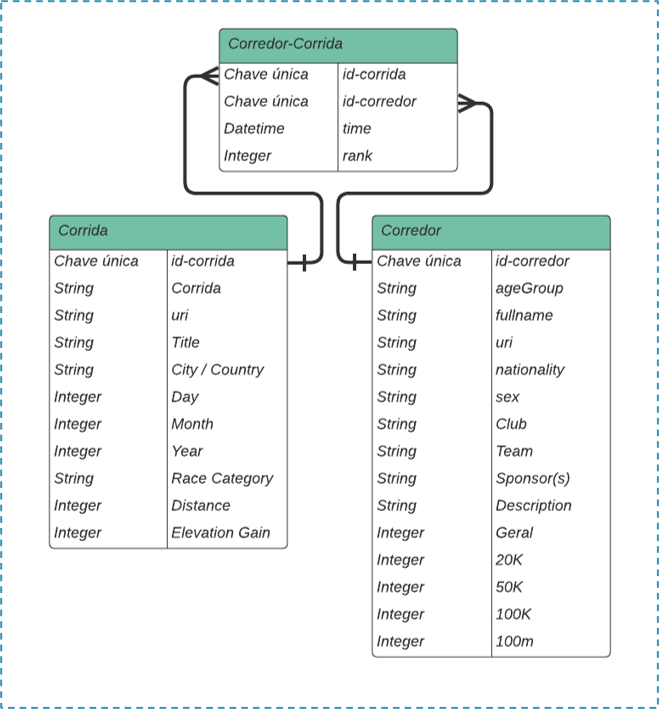
\includegraphics[width = 0.5\linewidth]{relatorios/paraty/figuras/ER_Data_Paraty.png}
    \label{fig:ER_Data_Paraty}
\end{figure}

A estrutura da base de dados inclui três tabelas principais: "Corredores", "Corridas" e "Corredor-Corrida" como apresentado na Figura \ref{fig:ER_Data_Paraty}. A tabela "Corredores" contém informações detalhadas sobre os participantes, incluindo identificador único, faixa de idade, nome completo, entre outras. Já a tabela "Corridas", armazena exclusivamente detalhes sobre os eventos de corrida, como identificador único, nome do evento, local, entre outros.

A tabela "Corredor-Corrida" estabelece o relacionamento entre corredores e corridas, registrando a participação de cada corredor em cada evento. Esta tabela contém o identificador da corrida (id-corrida), o identificador do corredor (id-corredor), o tempo do corredor na corrida (time) e o ranking do corredor na corrida (rank). Este relacionamento se organiza na forma de 1 para N dos dois lados da tabela, uma vez que um corredor corre múltiplas corridas, assim como uma corrida contém diversos corredores. Assim, a junção desses dados permite numerosas análises cruzando os dados de corredores e corridas, facilitando a extração de insights valiosos sobre o comportamento dos participantes e as características das corridas (Figura \ref{fig:ER_Data_Paraty}).

\section{Resultados}

Após a construção da base de dados por meio da técnica de Webscraping, foram realizadas diversas análises a partir dos dados extraídos.

\begin{figure}
    \centering
    \caption{Quantidade de corredores que participaram de corridas de corridas em cada ano}
    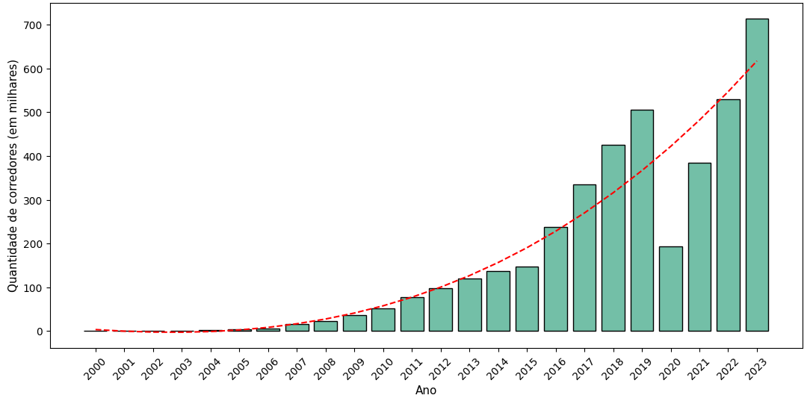
\includegraphics[width = 0.7\linewidth]{relatorios/paraty/figuras/Grafico_participantes.png}
    \label{fig:Participantes}
\end{figure}

A análise principal focou no crescimento do mercado de corridas de montanha. Conforme apresentado na Figura \ref{fig:Participantes}, observa-se um crescimento exponencial no número de corredores participantes ao longo dos anos, com exceção do período marcado pela pandemia de COVID-19. Esses resultados indicam que o mercado de corridas de montanha está em expansão, reforçando a relevância e o potencial deste estudo.

\subsection{Distribuição de Corredores de Montanha por Sexo}

O estudo da distribuição de corredores de montanha por sexo, representada na Figura \ref{fig:sexo}, revela uma predominância masculina no cenário atual. Dos corredores analisados, 24.090 são homens, enquanto 12.212 são mulheres, mostrando uma significativa diferença na participação entre os gêneros.

\begin{figure}
\centering
\caption{Distribuição de corredores de montanha brasileiros em atividade por sexo}
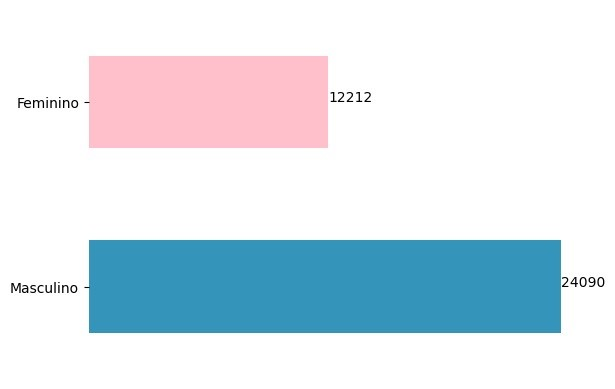
\includegraphics[width = 0.6\linewidth]{relatorios/paraty/figuras/Grafico_Corredores_Sexo.jpg}
\label{fig:sexo}
\end{figure}

Embora os homens constituam a maioria dos participantes, a presença expressiva de mulheres indica um nível considerável de diversidade nas corridas de montanha. Esses dados são valiosos para entender o perfil atual do mercado e podem ser utilizados para desenvolver estratégias específicas de inclusão e promoção voltadas para ambos os públicos, tanto masculino quanto feminino.

\subsection{Faixa de Idade dos Corredores Brasileiros}

A distribuição etária dos corredores de montanha brasileiros, ilustrada na Figura \ref{fig:corredores_idade}, apresenta uma tendência clara que segue um padrão semelhante ao de uma distribuição normal, porém ligeiramente deslocada para a esquerda.

\begin{figure}
\centering
\caption{Faixa de Idade dos Corredores Brasileiros}
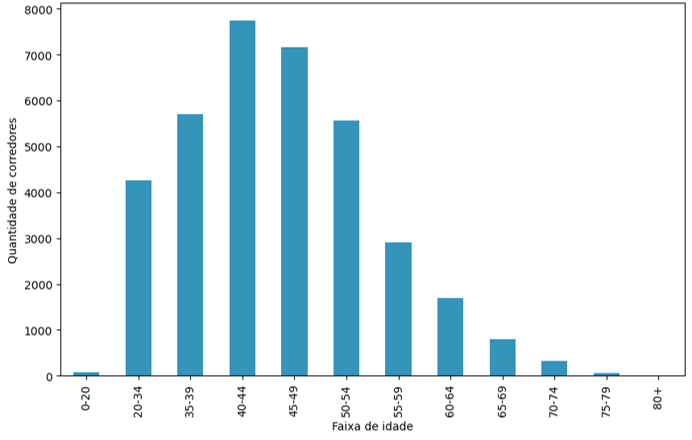
\includegraphics[width = 0.7\linewidth]{relatorios/paraty/figuras/Grafico_corredores_idade.png}
\label{fig:corredores_idade}
\end{figure}

Conforme o gráfico, observa-se uma baixa expressividade de corredores nas faixas etárias de 0 a 20 anos e acima dos 75 anos (particularmente nas faixas de 75-79 anos e 80+). Essas faixas indicam uma menor participação de jovens e idosos no cenário das corridas de montanha no Brasil.

Já nas faixas intermediárias, especialmente entre 55 e 74 anos, há uma participação de média expressividade. Esse grupo representa uma parcela considerável de corredores, mas sem o mesmo impacto numérico das faixas mais jovens.

A maior concentração de corredores está nas faixas etárias mais jovens e de meia-idade, variando entre 21 e 54 anos, que apresentam alta expressividade. Esses dados indicam que o perfil típico dos corredores de montanha no Brasil está centrado nas idades produtivas, com um foco particular na faixa dos 30 e 40 anos.

Essa análise permite uma melhor compreensão do público-alvo das corridas de montanha no país, destacando a necessidade de estratégias direcionadas a diferentes faixas etárias para incentivar a participação e retenção em cada grupo.



\section{Conclusão}

O estudo realizado sobre o mercado de corridas de montanha no Brasil mostrou que, apesar do crescimento dessa modalidade, ainda há uma falta de dados estruturados que possa sustentar o desenvolvimento de novas competições e o aprimoramento de estratégias de marketing e organização. Através da criação de uma base de dados estruturada, foi possível observar o crescente interesse por essa modalidade, bem como identificar as características demográficas dos participantes.

A análise dos dados revelou que o mercado está em expansão, com um número crescente de corredores participando de eventos ao longo dos anos. Além disso, a distribuição por sexo e faixa etária dos corredores fornece informações valiosas sobre o perfil dos participantes, o que pode ajudar na criação de estratégias mais eficientes de promoção e desenvolvimento do esporte.

Em termos de recomendações futuras, é crucial que mais pesquisas sejam realizadas para complementar os dados existentes, especialmente no que diz respeito a variáveis como os fatores que influenciam a escolha dos corredores por determinadas corridas, além da expansão de fontes de dados e a criação de uma plataforma centralizada para agregar informações sobre as corridas de montanha no Brasil.

Por fim, a construção da base de dados e a análise realizada fornecem uma base sólida para futuras investigações sobre o mercado de trail running no Brasil, permitindo uma compreensão mais profunda do comportamento dos corredores e as dinâmicas desse mercado emergente.

\subsection{Limitações}

As análises realizadas no presente projeto possuem algumas limitações e vieses que devem ser levados em consideração ao interpretar os resultados. Em primeiro lugar, a unilateralidade das fontes de dados utilizadas é um fator crítico. Todas as informações foram extraídas do site da UTMB, por meio de técnicas de web scraping, o que pode enviesar os resultados e limitar a representatividade dos dados. Dependendo do site, as informações podem não refletir completamente o universo dos corredores de montanha, deixando de lado dados de outros segmentos ou regiões não capturados por essa fonte.

Além disso, há uma questão de precisão e completude dos dados. A fonte utilizada pode não conter todas as informações relevantes para a análise, o que compromete a robustez dos resultados. Dados cruciais, como condições ambientais, variações regionais e detalhes sobre o perfil socioeconômico dos corredores, podem não estar disponíveis, o que limita a capacidade de realizar análises mais profundas ou identificar correlações importantes que poderiam surgir com fontes de dados mais amplas e diversas.

Outro ponto importante a ser considerado é a estrutura da página web. As páginas das quais os dados são extraídos podem sofrer alterações frequentes em seu layout ou na organização das informações. Isso pode, inevitavelmente, causar interrupções no processo de coleta de dados via web scraping, exigindo ajustes recorrentes no script e, em casos extremos, inviabilizando a extração dos dados. A manutenção contínua do código é um desafio que precisa ser monitorado ao longo do tempo.

Reconhecer essas limitações é fundamental para a interpretação cuidadosa dos resultados e para a busca de melhorias futuras no estudo.

\subsection{Passos futuros}

Para aprimorar a análise e aumentar a precisão dos dados, duas estratégias podem ser implementadas: a padronização da localidade das corridas e a expansão da base de dados.

Atualmente, os dados referentes à localidade das corridas e à nacionalidade dos corredores estão em formatos variados, como países, cidades, estados, coordenadas geográficas e outras designações. Para garantir a consistência e facilitar a análise, será implementada uma padronização dessas informações. Utilizaremos o Google Maps para converter e padronizar todas as localizações para o formato de cidades.

Essa padronização não só melhorará a qualidade dos dados, mas também permitirá uma análise mais coesa e comparativa das informações. Com a localidade padronizada, será possível identificar padrões e tendências de forma mais eficaz, além de comparar dados de diferentes regiões com maior precisão.

Ainda, para enriquecer ainda mais o estudo, planejamos expandir a base de dados para incluir dados de corredores de todas as nacionalidades cadastrados na Ultra-Trail du Mont-Blanc (UTMB), e não apenas corredores brasileiros.

A coleta desses dados globais pode levar aproximadamente 30 dias e envolve a obtenção de informações de cerca de 2,75 milhões de corredores. Esta expansão permitirá analisar tendências e padrões não apenas no Brasil, mas também em uma escala internacional, proporcionando insights valiosos sobre o perfil dos corredores de montanha ao redor do mundo. A inclusão desses dados ampliará a compreensão das características demográficas, preferências e comportamentos dos corredores em diferentes regiões, oferecendo uma análise mais completa e representativa do mercado global de corridas de montanha.

% \section{Referências}

% \begin{thebibliography}{9}

% \bibitem{oliveira2017} 
% OLIVEIRA JUNIOR, Daniel Ramos. \textit{Mercado do trail running no Paraná: análise dos agentes estruturantes responsáveis pelo desenvolvimento da modalidade}. 2017. 45 f. Trabalho de Conclusão de Curso (Graduação) – Curso de Bacharelado em Educação Física. Universidade Tecnológica Federal do Paraná. Curitiba. 2017. Disponível em: \url{https://repositorio.utfpr.edu.br/jspui/bitstream/1/7876/1/CT_COEFI_2017_1_03.pdf}. Acesso em: 24 fev. 2024.

% \bibitem{utmb2023}
% ULTRA TRAIL DU MONT BLANC. Electric atmosphere at first ever Paraty Brazil by UTMB, as Rogério Silvestrin and Giovanna Martins win queen stage and qualify for UTMB World Series Finals. 2023. Disponível em: \url{https://utmb.world/news/results-Paraty-Grindstone-next-event-Nice}. Acesso em: 24 fev. 2024.

% \bibitem{utmb2016}
% ULTRA TRAIL DU MONT BLANC. Trans Peneda Gerês 2016 - Trail World Championships 2016. Disponível em: \url{https://utmb.world/utmb-index/races/5483.transpenedagerestrailworldchampionships.2016?page=1}. Acesso em: 24 fev. 2024.

% \bibitem{fogliato2020}
% Fogliato, Riccardo; Oliveira, Natalia L.; Yurko, Ronald. \textit{TRAP: A Predictive Framework for Trail Running Assessment of Performance}. 4 de fevereiro de 2020. Disponível em: \url{https://arxiv.org/abs/2002.01328}. Acesso em: 24 fev. 2024.

% \bibitem{utmbparaty}
% ULTRA TRAIL DU MONT BLANC. Paraty Brazil by UTMB. Disponível em: \url{https://paraty.utmb.world/pt}. Acesso em: 24 fev. 2024.

% \bibitem{hague2021}
% HAGUE, Paul; HARRISON, Matthew; CUPMAN, Julia; TRUMAN, Oliver. *Market Research in Practice*. 4. ed. Kogan Page, 2021.

% \bibitem{findarunner}
% INTERNATIONAL TRAIL RUNNING ASSOCIATION. Find a Runner. Disponível em: \url{https://itra.run/Runners/FindARunner}. Acesso em: 24 dez. 2024.


% \end{thebibliography}


\printbibliography[keyword = paraty]

